\subsection{Infraestructura y herramientas}
\subsubsection{Descripción general de la infraestructura}
La infraestructura y las herramientas son la base sobre la que se construirán
los diferentes proyectos de aprendizaje automático. Se encargan de proporcionar
un entorno de desarrollo e investigación eficiente, que permita a los miembros
del equipo centrarse en el desarrollo de modelos sin tener que preocuparse por
la configuración. Concretamente, se han desplegado dos plataformas integradas
que vienen a cubrir varias de las necesidades fundamentales de los proyectos
como son la gestión de dataset, la monitorización de experimentos o la
exploración de datasets. Además, se ha añadido un sistema de autenticación 
para garantizar la seguridad y privacidad de los datos.\medskip

Esta infraestructura se ha desplegado en un servidor interno de la empresa
utilizando contenedores de Docker. La elección de esta tecnología se debe a
que permite la creación de entornos aislados y portables, lo que facilita el
despliegue de las aplicaciones. Se ha utilizado Docker Compose para
sincronizar el despliegue de los diferentes servicios, lo que permite
realizar despliegues automatizados mediante las acciones de GitLab CI. La
figura \ref{fig:internal-server} muestra una vista general de la infraestructura
desplegada en el servidor interno de la empresa. En ella se pueden observar
los diferentes servicios desplegados y cómo se comunican entre ellos. Además,
se puede observar que todos los servicios están interconectados mediante un
proxy inverso mediante Nginx que se encarga de redirigir las peticiones en 
función de la URL de la petición. Esto permite que todos los servicios sean
accesibles desde el exterior a través de un único punto de entrada y que el
sistema de autenticación sea común para todos los servicios.

\begin{figure}[ht]
    \centering
    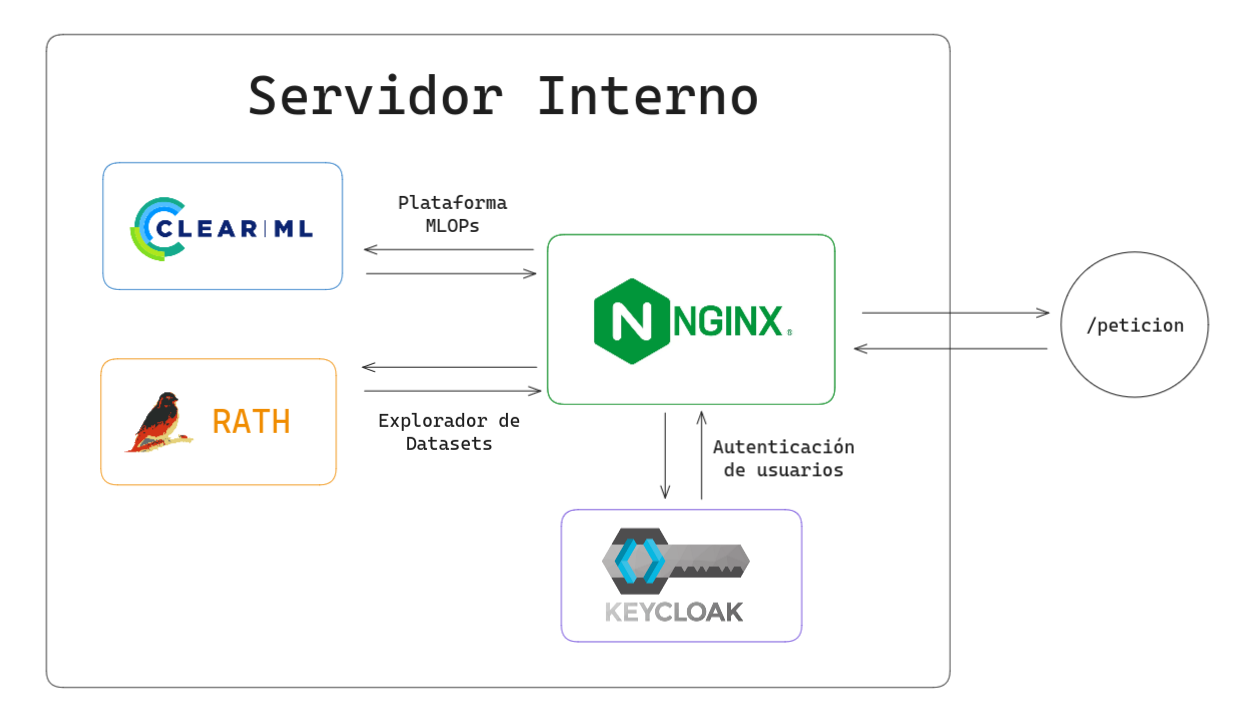
\includegraphics[width=\textwidth]{internal-server.png}
    \caption{Vista general del proyecto}\label{fig:internal-server}
\end{figure}

\subsubsection{Plataformas integradas}


\subsubsection{Herramientas de desarrollo}
\subsubsection{Seguridad y priviacidad}
\subsubsection{Despligue Automatizado}